\documentclass[a4paper]{memoir}
\usepackage[utf8]{inputenc}
\usepackage[frenchb]{babel}
\usepackage{graphicx}
\usepackage{float}
\usepackage{hyperref}
\usepackage{verbatim}
\usepackage{enumitem}
\usepackage[babel=true]{csquotes}

\pagestyle{plain}

\title{\textbf{Rapport de projet}\\- \Huge{OpenSculpt} -}
\author{\emph{GAUTHIER Silvère}\\\emph{LAMEIRA Yannick}\\\emph{PELADAN Cécile}}
\date{\today}

\begin{document}
	\maketitle
	\newpage
	\tableofcontents

	\chapter{Remerciements}

		Un grand merci à Frédéric Boudon et Benjamin Gilles pour leur encadrement.

	\chapter{Introduction}
		
		\section{Sujet initial}
				L'objectif de ce projet est de créer un logiciel de sculpture 3D. L'utilisateur aurait à disposition un maillage déformable, qu'il pourrait modeler avec différents outils tels que déplacement, extrusion de matière ou lissage. L'interface devra permettre à l'utilisateur de facilement créer un maillage initial, le visualiser et interagir avec lui à l'aide des différents outils de modelage.

	Initialement, les premières fonctionnalités à implémenter seront la création d'une sphère ou
d'un cube comme maillage de départ, la navigation dans l'espace 3D pour se positionner autour du maillage, puis les outils de déformations cités ci-dessus. Une interface graphique contenant les
boutons d'outils sera définie pour que l'utilisateur puisse intuitivement appliquer les différentes opérations proposées.

	Les principales difficultés ici seront d'abord de gérer correctement l'interaction 3D de l'utilisateur avec le maillage via le curseur et la fenêtre 2D. Ensuite viendra la mise en place d'une structure de données efficace et robuste de maillage avec l'implémentation des algorithmes de subdivision et de raffinement.

	Si le temps le permet, d'autres outils et maillages de base pourront être implémentés, afin
d'enrichir le logiciel. On pourra également réfléchir à une manière d'importer et exporter les
maillages sous différents formats tels que le OBJ ou le STL par exemple.

	Ce logiciel sera développé en C++ avec la bibliothèque OpenGL pour le rendu 3D et la bibliothèque Qt par pour définir l'interface.
	
	\chapter{Cahier des charges}
		Ce chapitre détaille toute la phase de conception du projet.
	
		\section{Questions fréquentes}
			Cette partie regroupe les caractéristiques basiques de l'application sous forme de question-réponse.
		
			\subsection{... ?}
				
			\subsection{... ?}
				
			
		\section{Mécanismes}
			Cette section détaille succintement les fonctionnalités disponibles.
			
			\subsection{Les Modèles}
				cube, sphère, cylindre, tore… (avec paramètres modifiables)

			\subsection{Les Outils de sculpture}
				extrusion, intrusion, lissage, déplacement, gonflement, pincement...

			\subsection{Les Outils de modélisation}
				symétrie axiales et centrales, subdivision, simplification, (union, différence), déplacement, rotation et mise à l'échelle de l'objet, fils de fer / solide, (validation maillage)

			\subsection{Interface}
				déplacement, rotation et zoom dans la fenêtre OpenGL, boites d'outils, menus déroulants, boutons, afficher la grille / le repère, perspective

			\subsection{Les Options}
				nouveau, ouvrir, enregistrer, importer, exporter, annuler, refaire, paramètres, quitter
		
			\subsection{Autres}
				matériaux, lumière
	
		\section{Structure du programme}
			Cette partie détaille succintement la structure globale du logiciel, ce qui couvre les aspects non maîtrisables par l'utilisateur.
			
			\subsection{...}
				
			
		\section{\'Eléments graphiques}
			\subsection{Interface utilisateur}
				
		
		
	\chapter{Gestion du projet}
		Cette partie traite globalement de tout ce qui concerne l'organisation du projet, que ce soit au niveau de la conception, du développement, de l'équipe ou encore de la gestion des fichiers.
		
		\section{Gestion de l'équipe}
			Tous les membres se connaissant et étant supposés être capable de travailler en équipe, nous n'avons fait aucune élection de chef de projet.\\
			Nous avons opté pour travailler de manière collégiale, et ainsi garder une cohésion de groupe sans pour autant avoir de hiérarchie instaurée au sein du groupe, qui pourrait au contraire déservir la réalisation de nos objectifs.\\
			Chaque membre a donc autant de pouvoir que les autres, et peut donc participer activement au projet, autant lors de la conception que du développement. Toutes les décisions seront prises suivant la majorité lors de votes.\\\\
			Pour ce qui est des réunions de projets, nous avons convenu avec nos tuteurs d'une réunion, allant d'environ trente minutes à une heure, toutes les semaines, afin de mettre au point l'avancement du projet. En parallèle, tous les membres de notre équipe se retrouvent une fois par semaine afin de discuter des points clés effectués ou à venir, donner lieu aux votes pour les prises de décisions, ou encore, lors de la phase de développement, travailler en collaboration afin d'optimiser notre travail.\\\\
			Au niveau du travail collaboratif, nous avons mis en place un dépôt sur github (adresse à la page \pageref{url:github}), contenant tant la documentation que les sources de notre jeu. Par ailleurs, nous mettrons sur ce dépôt uniquement les fichiers sources, les images et les sons, mais en aucun cas les fichiers temporaires ou les exécutables. Les seuls fichiers binaires disponibles seront les PDF de la documentation, pour un soucis de facilité d'accès.

		\section{Découpage en tâches}
			Afin de préparer le développement du programme, il était nécessaire de séparer les fonctionnalités les unes des autres. Nous avons abouti à ce diagramme, qui résume notre choix de découpage :\\
			\begin{figure}[H]
				\begin{center}
					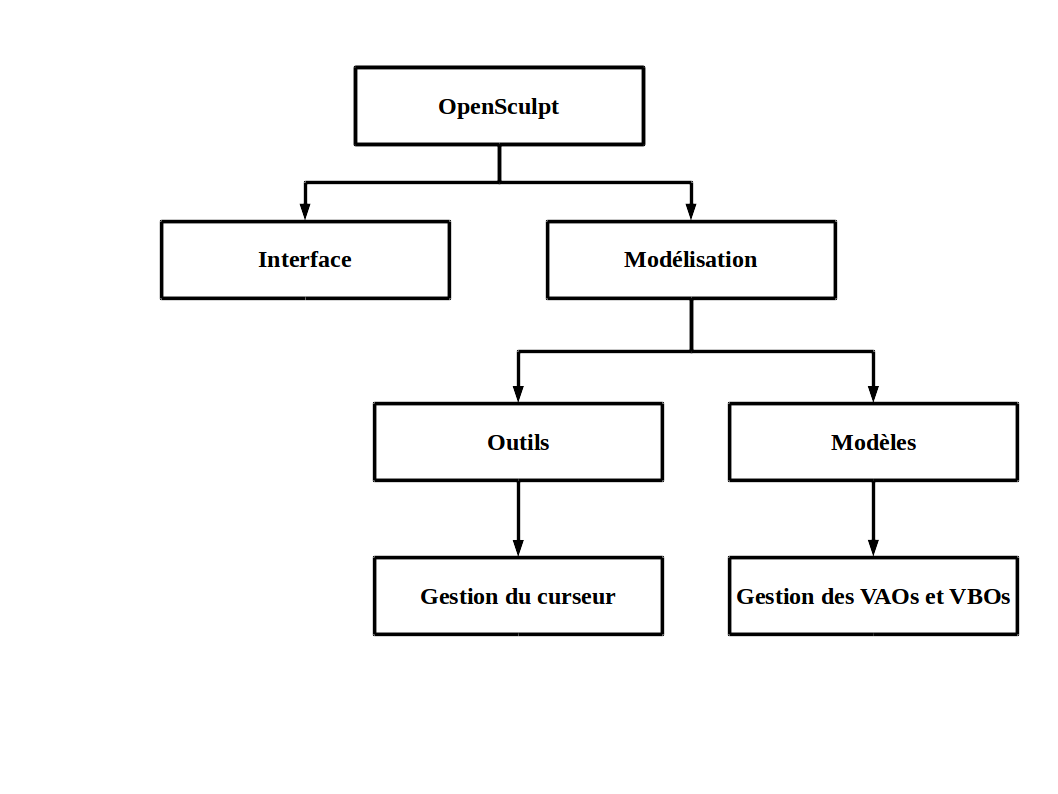
\includegraphics[scale=0.5]{img/DiagrammeDecoupageProjet.png}
				\end{center}
				\label{fig:decoupage}
				\caption{Diagramme des tâches du projet}
			\end{figure}

		\section{Assignation}
			Le projet étant découpé en un certain nombre de modules, il ne restait plus qu'à assigner chaque tâche à un ou plusieurs membres de l'équipe. Nous nous sommes organisés comme ceci :
			\begin{itemize}[label=$\bullet$]
				\item \textbf{Mise en place de l'interface} : LAMEIRA Yannick.
				\item \textbf{Outils et gestion du curseur} : PELADAN Cécile.
				\item \textbf{Modèles et gestion des VAOs et VBOs} : GAUTHIER Silvère.
			\end{itemize}
			Bien entendu, cette répartition n'est pas totalement fixée, elle concerne en réalité l'affectation de responsables de parties, qui seront en charge de celle-ci mais pourront évidemment faire appel aux autres membres pour trouver une solution à un problème par exemple.\\
			Le détail complet des tâches et assignations se situe dans la section Gestion du temps, page \pageref{GestionTps}.

		\section{Gestion du temps}
			\label{GestionTps}
			Afin de clarifier notre gestion du temps, un diagramme de Gantt est disponible en annexe (cf page \pageref{fig:Gantt} et dans la documentation de notre projet, et sera mis à jour en fonction de l'avancée du projet.\\

		\section{Choix technologiques}
			Afin de pouvoir développer correctement notre logiciel, il a fallu définir tout ce que nous allions utiliser en terme de langages et bibliothèques selon notre logique de conception.
			
			\subsection{Langages de programmation}
				Pour des besoins de performances, nous avons comparé différents langages. Pour réduire le temps de recherche et de comparaison, nous nous sommes appuyé sur des tests déjà effectués par d'autre.\\
				Des tests de performances concernant un large panel de langages, comparés dans quatre contextes différents, sont fournis en annexe, page \pageref{fig:analyse}.\\
				Nous pouvons observer que globalement, le langage le plus rapide est ici C++. L'utilisation de ce langage étant très fréquente dans les applications en temps réel, de part sa réputation d'un des langages les plus performants, et tous les membres de notre équipe sachant l'utiliser, nous avons fait le choix de programmer le logiciel en C++.\\

			\subsection{Bibliothèques}
				Pour la gestion graphique de l'interface et de l'affichage de l'objet, nous avons cherché une bibliothèque relativement simple d'utilisation mais surtout performante afin de garder la fluidité gagnée avec le choix des langages de programmation.\\
				Connaissant la bibliothèque OpenGL, qui est bas niveau et performante dans les affichages deux et trois dimensions, nous nous sommes tournés vers une bibliothèque utilisant OpenGL : Qt.\\

			\subsection{Représentation du maillage}
				Nous cherchons ici à comparer différentes techniques permettant de représenter un maillage, afin de choisir celle qui sera la plus adaptée à nos opérations. Voici un tableau récapitulatif de cette étude comparative :
				\begin{table}[H]
					\begin{small}
						\begin{tabular}{| c | l | l |}
							\hline
							\textbf{Représentation} & \textbf{Avantages} & \textbf{Inconvénients}\\
							\hline
							 & - Hiérarchie des résolutions & - Visualisation surfacique difficile\\
							Octree ou KDTree & - Rendu volumique possible & - Coût de stockage excessif\\
							 & - Construction et parcours simples & - Recalculer à chaque modification\\
							\hline
							 & - Historique de construction & - Non unicité\\
							Arbre CSG & - Approche fonctionnelle & - Opérations complexes\\
							 &  & - Domaine insuffisant\\
							\hline
							G-maps & - Opérations de topologie simples & - Séparation topologie / plongement\\
							 & - Plongements multiples & \\
							\hline
							Liste de triangles & - Opérations simples & - Stockage non optimisé\\
							\hline
							Sommets partagés & - Opérations simples & \\
							 & - Stockage correct & \\
							\hline
							Bandes de triangles & - Stockage correct & - Chaque sommet est visité deux fois\\
							 &  & - Opérations de déplacement délicates\\
							\hline
							Structure par faces & - Chaque face pointe sur ses sommets & - Pas d'accès direct aux arêtes\\
							 & - Une face connaît les faces adjacentes & \\
							\hline
							Structure par demi-arêtes & - Parcours de maillage très pratiques & - Coût de stockage excessif\\
							\hline
							Vertex Array (VAO) & - Optimisé pour le rendu OpenGL & - Utilise le CPU et la RAM\\
							 & - Simple d'utilisation & \\
							\hline
							Vertex Buffer Object (VBO) & - Optimisé pour le rendu OpenGL & \\
							 & - Utilise le GPU et la VRAM & \\
							\hline
						\end{tabular}
					\end{small}
					\label{tab:maillage}
					\caption{Tableau comparatif de méthodes de représentation de maillage 3D}
				\end{table}
				L'étude comparative montre qu'il serait judicieux d'utiliser conjointement des Vertex Buffer Objects (VBOs) afin d'optimiser les performances et une classe personnalisée pour aisément gérer nos données par une surcouche de méthodes.
			
		\section{Gestion des fichiers}
			Nous avons beaucoup de fichiers à gérer dans ce projet, et nous devions établir des conventions ou des moyens afin de les gérer correctement.
			
			\subsection{Format des Fichiers}
				Le code étant écrit en C++, nous utiliserons des fichiers d'en-tête au format HPP et des fichiers de définition au format CPP.\\
				Toutes les images nécessaires au jeu seront au format PNG afin de pouvoir utiliser la transparence et garder la pleine qualité d'image (contrairement à JPEG qui perd de l'information à la compression).\\
			
				\subsubsection{Sauvegarde}
					Un fichier sera créé pour la sauvegarde de l'objet en cours.\\
			
			\subsection{Commentaires}
				Si une méthode ou fonction, voir même un bloc, dépasse une certaine taille ou devient trop compliquée, un commentaire sera ajouté avant celle-ci expliquant brièvement son processus :
				\begin{verbatim}
					/** Description :
					*** Entrée : ...
					*** Sortie : ...
					**/
				\end{verbatim}
				Quelque commentaires précieux pour le travail collaboratif seront également présents :
				\begin{table}[H]
					\begin{small}
						\begin{tabular}{| c | c |}
							\hline
							\textbf{Marqueur spécifique} & \textbf{Signification}\\
							\hline
							TODO & \'A mettre à la place du code d'une fonctionnalité à implémenter\\
							\hline
							RECODE & \'A mettre au dessus du bloc d'une fonctionnalité à refaire ou à optimiser\\
							\hline
							FIXME & \'A mettre au dessus du bloc d'une fonctionnalité contenant un bug\\
							\hline
						\end{tabular}
					\end{small}
					\label{tab:commentaire}
					\caption{Forme et usage des commentaires}
				\end{table}

			\subsection{Conventions de Nommage}
				Pour la lisibilité et la bonne pratique du développement de l'application, il est nécessaire de suivre des règles établies au sein de l'équipe de projet, appelées conventions. Ainsi, nous avons choisi d'écrire le code en anglais uniquement, mis à part pour les commentaires utiles aux développeurs préférant le français. De même, au moins une ligne de commentaire est requise avant chaque déclaration de classe ou de fonction, afin d'en expliquer brièvement son fonctionnement.\\
				Enfin, nous avons choisi de faire précéder le nom de chacune de nos classes par \enquote{OS} pour \enquote{OpenSculpt}. Les noms des classes seront alors de la forme \enquote{OS\textit{NomClasse}}. De la même manière, les noms des variables seront de la forme \enquote{m\_\textit{nomVariable} } pour les attributs de classe, \enquote{g\_\textit{nomVariable} } pour les variables globales et \enquote{s\_\textit{nomVariable} } pour les variables statiques.
				
				\begin{table}[H]
					\begin{small}
						\begin{tabular}{| c | c |}
							\hline
							\textbf{Type de variable} & \textbf{Format du nom}\\
							\hline
							Classe & Majuscule suivit de minuscules\\
							 & Précédé par OS\\
							\hline
							Méthode & Minuscules (pour les mots composés,\\
							et & chaque mots suivant est\\
							Fonction & une majuscule suivit de minuscules)\\
							\hline
							Attribut de classe & Précédé par m\_\\
							\hline
							Variable globale & Précédé par g\_\\
							\hline
							Variable statique & Précédé par s\_\\
							\hline
						\end{tabular}
					\end{small}
					\label{tab:nommage}
					\caption{Conventions de nommage}
				\end{table}

			\subsection{Gestion du code source}
				Afin de faciliter le travail collaboratif, nous utilisons un dépôt utilisant le gestionnaire de version GIT, hébergé sur le site :
				\begin{center}
					\url{https://github.com/slvrgauthier/OpenSculpt}
					\label{url:github}
				\end{center}
				Sur ce dépôt seront présents tous les fichiers sources nécessaires au développement du programme ainsi que les documentations au format \LaTeX, ODT et PDF (même si aucun fichier binaire ne devrait être présent, il est plus pratique de récupérer directement un tel fichier que de le compiler soit-même). De plus, y seront stockées toutes les données utilisées par le programme telles que les images et autres ressources. Seuls les fichiers temporaires, exécutables et fichiers de sauvegarde ne seront pas stockés.


	\chapter{Développement}
		Ce chapitre est une sorte de carnet de bord. Il détaille tout ce qui concerne le développement de l'application.
		
		\section{...}
			
		
			\subsection{...}
				
			
	\chapter{Post-Mortem}
		Cette section liste toutes les étapes de la conception que nous n'avons pas réalisées (selon notre ordre de priorités), ainsi que toutes les améliorations auxquelles nous avons pensé lors de la phase de développement.
		
		\section{Fonctionnalités non implémentées}
			
			
		\section{Améliorations réalisables}
			
	
	\appendix
	\chapter{}
		Dans cette partie seront placés les éléments trop volumineux pour être inclus directement dans le texte, tels que les images ou graphiques.\\
		
		\section{Diagramme de Gantt}
			Le diagramme est fourni page \pageref{fig:gantt}.
			
		\section{Comparatif de performances}
			Le graphique est situé page \pageref{fig:analyse}.
			
		\section*{}
			\begin{figure}
				\vspace{-3,5cm} \hspace{-4,5cm} 
\includegraphics[scale=0.6]{img/Gantt.png}
				\label{fig:gantt}
				\vspace{-0,5cm} \caption{Diagramme de Gantt}
			\end{figure}
			
			\begin{figure}
				\begin{center}
					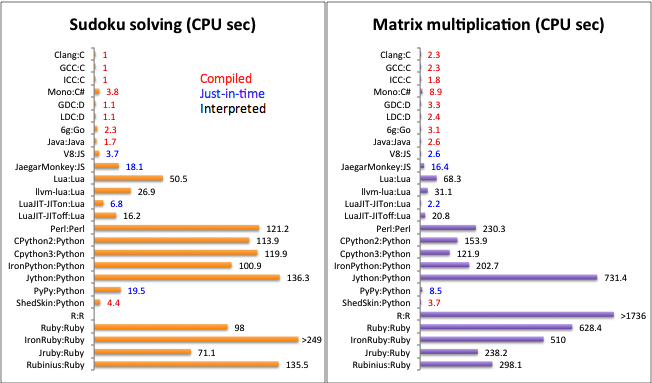
\includegraphics[scale=0.5]{img/AnalyseLangage1.png}
					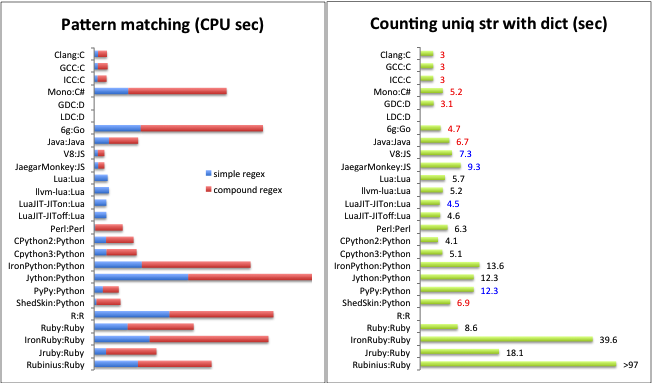
\includegraphics[scale=0.5]{img/AnalyseLangage2.png} 
				\end{center}
				\label{fig:analyse}
				\caption{Comparaisons de performances de divers langages dans des cas donnés}
				Source : \url{http://attractivechaos.wordpress.com/2011/06/22/my-programming-language-benchmark-analyses/}
			\end{figure}

\end{document}
